\documentclass[]{elsarticle} %review=doublespace preprint=single 5p=2 column
%%% Begin My package additions %%%%%%%%%%%%%%%%%%%
\usepackage[hyphens]{url}

  \journal{Ecology Letters} % Sets Journal name


\usepackage{lineno} % add
\providecommand{\tightlist}{%
  \setlength{\itemsep}{0pt}\setlength{\parskip}{0pt}}

\usepackage{graphicx}
\usepackage{booktabs} % book-quality tables
%%%%%%%%%%%%%%%% end my additions to header

\usepackage[T1]{fontenc}
\usepackage{lmodern}
\usepackage{amssymb,amsmath}
\usepackage{ifxetex,ifluatex}
\usepackage{fixltx2e} % provides \textsubscript
% use upquote if available, for straight quotes in verbatim environments
\IfFileExists{upquote.sty}{\usepackage{upquote}}{}
\ifnum 0\ifxetex 1\fi\ifluatex 1\fi=0 % if pdftex
  \usepackage[utf8]{inputenc}
\else % if luatex or xelatex
  \usepackage{fontspec}
  \ifxetex
    \usepackage{xltxtra,xunicode}
  \fi
  \defaultfontfeatures{Mapping=tex-text,Scale=MatchLowercase}
  \newcommand{\euro}{€}
\fi
% use microtype if available
\IfFileExists{microtype.sty}{\usepackage{microtype}}{}
\usepackage[margin=1.1in]{geometry}
\bibliographystyle{elsarticle-harv}
\usepackage{longtable}
\ifxetex
  \usepackage[setpagesize=false, % page size defined by xetex
              unicode=false, % unicode breaks when used with xetex
              xetex]{hyperref}
\else
  \usepackage[unicode=true]{hyperref}
\fi
\hypersetup{breaklinks=true,
            bookmarks=true,
            pdfauthor={},
            pdftitle={Quantifying mesopredator release: lethal control of an invasive apex predator alters feral cat density and detectability},
            colorlinks=false,
            urlcolor=blue,
            linkcolor=magenta,
            pdfborder={0 0 0}}
\urlstyle{same}  % don't use monospace font for urls

\setcounter{secnumdepth}{5}
% Pandoc toggle for numbering sections (defaults to be off)

% Pandoc citation processing

% Pandoc header
\usepackage{setspace}\doublespacing
\usepackage{float}
\floatplacement{figure}{H}



\begin{document}
\begin{frontmatter}

  \title{Quantifying mesopredator release: lethal control of an invasive apex predator alters feral cat density and detectability}
    \author[UOM]{Matthew W. Rees\corref{1}}
   \ead{matt.wayne.rees@gmail.com} 
    \author[CEC]{Jack H. Pascoe}
  
    \author[CEC]{Mark Le Pla}
  
    \author[ARI]{Alan Robley}
  
    \author[CEC]{Emma K. Birnbaum}
  
    \author[UOM]{Brendan A. Wintle}
  
    \author[UOM]{Bronwyn A. Hradsky}
  
      \address[UOM]{Quantitative \& Applied Ecology Group, School of Ecosystem and Forest Science, The University of Melbourne, Parkville, VIC, Australia}
    \address[CEC]{Conservation Ecology Centre, Otway Lighthouse Rd, Cape Otway, VIC, Australia}
    \address[ARI]{Department of Environment, Land, Water and Planning, Arthur Rylah Institute for Environmental Research, Heidelberg, Australia}
      \cortext[1]{Corresponding Author}
  
  \begin{abstract}
  
  \end{abstract}
   \begin{keyword} camera trap; \emph{Felis catus}; invasive predator; interspecific competition; mesopredator release; population density; spatial capture-recapture; spatial mark-resight; species interactions; \emph{Vulpes vulpes}.\end{keyword}
 \end{frontmatter}

\parskip=12pt

\newpage

\hypertarget{abstract}{%
\section*{ABSTRACT}\label{abstract}}
\addcontentsline{toc}{section}{ABSTRACT}

The mesopredator release hypothesis predicts that subordinate predator density increases following apex predator decline. We replicated field experiments across two regions with a simple predator guild comprising the introduced red fox \emph{Vulpes vulpes} and feral cat \emph{Felis catus}. We identified 160 individual cats from 68,504 camera-trap nights and estimated cat density with spatial mark-resight models. Lethal fox control increased cat density at a landscape-scale. Effect sizes ranged from negligible to a 3.7-fold increase in cat density, mirroring variation in the duration and intensity of fox suppression. At a fine-spatial scale, feral cat density was negatively associated with fox occurrence, suggesting integrated predator management would help protect shared native prey. Nonlinear models indicated cats exhibited avoidance behaviour when foxes were rare, but declined in density when fox activity was high. Mesopredator release can manifest as changes in both behaviour and density, distorting inference if these processes are not distinguished.

\newpage

\hypertarget{introduction}{%
\section{INTRODUCTION}\label{introduction}}

Understanding species interactions is critical for effective invasive species management (Zavaleta \emph{et al.} 2001). When several invasive species co-occur, management actions that suppress the dominant invasive species may inadvertently benefit subordinate invasive species (Jackson 2015; Kuebbing \& Nuñez 2015). For example, the removal of a dominant invasive predator may increase the abundance of a subordinate invasive species directly by reducing top-down pressure or indirectly by increasing in the availability of shared resources; these are often referred to as mesopredator or competitor release, respectively (Crooks \& Soulé 1999; Ruscoe \emph{et al.} 2011; Doherty \& Ritchie 2017). The release of subordinate invasive species, particularly predators, can have serious negative implications for native taxa and ecosystem function (Courchamp \emph{et al.} 1999; Ballari \emph{et al.} 2016). However, integrated invasive predator management is often far more costly and less feasible than single species control, and so it is important to identify when the extra cost is justified (Bode \emph{et al.} 2015).

Most knowledge of predator interactions stems from unreplicated `natural experiments' (e.g.~range contractions - Crooks \& Soulé 1999) or ad-hoc management interventions (e.g.~invasive species eradications - Rayner \emph{et al.} 2007). However, the occurrence, nature (positive or negative, direct or indirect) and strength of species interactions can vary among species assemblages, predation risk, environmental productivity, management regimes and other landscape contexts (Hastings 2001; Finke \& Denno 2004; Alston \emph{et al.} 2019). Replicating management programs in an experimental framework is logistically challenging, but important for understanding these complexities, discriminating between plausible hypotheses and producing generalisable results to inform effective pest management (Glen \& Dickman 2005; Christie \emph{et al.} 2019; Smith \emph{et al.} 2020).

Another source of uncertainty around the mesopredator release hypothesis stems from the inability of traditional survey and modelling approaches to distinguish behavioural from numerical population processes (Hayward \emph{et al.} 2015; Stephens \emph{et al.} 2015). Suppression of an apex predator may simultaneously change the behaviour and the density of a mesopredator, both of which influence detection rates (Broadley \emph{et al.} 2019; Rogan \emph{et al.} 2019). This makes it difficult to interpret observed changes in naive indices of mesopredator activity or occupancy in relation to changes in apex predator populations, even if the study has an experimental design. Unbiased estimates of invasive predator density are also important for setting meaningful control targets and to infer impacts on native prey (Moseby \emph{et al.} 2019). Spatial capture-recapture methods offer a solution by separating behavioural and observational processes from population density, estimated within a defined spatial resolution (Borchers \& Efford 2008).

Predation by two invasive species, the red fox \emph{Vulpes vulpes} (hereafter `foxes') and feral cat \emph{Felis catus} (hereafter `cats'), has played a major role in Australia's high rates of mammalian extinction (Woinarski \emph{et al.} 2015). Integrated management programs for these species are rare; instead, foxes are far more commonly controlled than cats, as they are more susceptible to poison-baiting, have greater direct economic impacts and fewer legal impediments to control (Reddiex \emph{et al.} 2007; McLeod \& Saunders 2014). Nonetheless, cats are one of the most widespread and damaging vertebrate predator species (Medina \emph{et al.} 2011; Doherty \& Ritchie 2017; Legge \emph{et al.} 2020). As foxes are larger-bodied (\textasciitilde2 kg difference) and have high dietary overlap with cats (Stobo-Wilson \emph{et al.} 2021a, b), the mesopredator release hypothesis (Soulé \emph{et al.} 1988) predicts that the impacts of cats on shared prey species will increase as fox populations are suppressed. This is alarming because feral cats are extremely difficult to manage in open populations (Fisher \emph{et al.} 2015; Lazenby \emph{et al.} 2015).

Evidence that foxes suppress cats is inconclusive (Hunter \emph{et al.} 2018). In parts of Australia where the native apex mammalian predator (the dingo \emph{Canis familiaris}) is functionally extinct and introduced foxes are the largest terrestrial mammalian predator, four studies have observed an increase in cat detections following fox control (Risbey \emph{et al.} 2000; Marlow \emph{et al.} 2015; Stobo-Wilson \emph{et al.} 2020). However, two other studies in similar systems did not see any change (Towerton \emph{et al.} 2011; Molsher \emph{et al.} 2017). A further study with spatial replication detected an increase at one site but not another (Davey \emph{et al.} 2006), and another observed a decrease in cat activity (Claridge \emph{et al.} 2010). No prior studies have directly estimated cat density in response to fox control.

We experimentally investigated the role of introduced foxes in top-down suppression of cat density in two regions of south-eastern Australia. Our experiments had a replicated Control-Impact design in the region with long-term fox control, and a Before-After Control-Impact Paired Series (BACIPS) design in the region with newly implemented fox control. Foxes and cats are the only functional terrestrial mammalian predators in these regions, and each region included at least one area in which foxes were subject to continuous lethal poison-baiting (hereafter `impact landscape'), and a paired area where foxes were not controlled (hereafter `non-impact landscape'). This allowed a sharp focus on the interactions between the two invasive predators, across a gradient of apex predator (fox) occurrence. In accordance with the mesopredator release hypothesis, we predicted that: (1) cat density would be negatively correlated with fox occurrence at a fine spatial scale, and (2) fox control would increase cat density at a landscape scale. We based inference on direct estimates of cat density using spatially explicit mark-resight models.

\newpage

\hypertarget{materials-and-methods}{%
\section{MATERIALS AND METHODS}\label{materials-and-methods}}

\hypertarget{study-area}{%
\subsection{Study area}\label{study-area}}

We conducted our study across two regions of south-west Victoria, Australia (Fig. \ref{fig:map}). The native temperate forests in both regions are fragmented to varying degrees, primarily by livestock farming and tree plantations. Although once widespread, native dingoes are now absent throughout, and a native mesopredator, the tiger quoll \emph{Dasyurus maculatus} is long absent from the Glenelg region and extremely rare in the Otway Ranges (last sighted in 2014 despite extensive camera-trapping). The terrestrial mammalian predator guild is therefore depauperate, with foxes and cats being the primary functional mammalian terrestrial predators; birds of prey and snakes are the only other medium-large carnivores present.

Our study landscapes in the Glenelg region, Gunditjmara country, were primarily lowland forest and heathy woodland. The area receives an average annual rainfall of 700 mm (``Bureau of meteorology'' 2021) and has gently undulating terrain. The region frequently experiences prescribed burns and wildfires, creating a mosaic of fire histories and vegetation complexity. Our study landscapes in the Otway region were in the western section of the Otway Ranges on Gadubanud country. Rainfall here is more than twice as high as the Glenelg region. The vegetation is a mosaic of shrubby wet forest and cool temperate rainforest, with our northern sites bordering on a large heathy woodland. This region rarely experiences fire and is nearly ten times more rugged than the Glenelg region (based on the terrain ruggedness index; Riley \emph{et al.} 1999).

Government land managers conduct ongoing targeted fox control for biodiversity conservation across broad sections of each region. In these sections, manufactured poison baits (FoxOff, Animal Control Technologies, Somerton) containing 3 mg of sodium mono-fluroacetate (1080) are buried at a depth of 12-15 cm at 1-km intervals along accessible forest tracks and roads (Fig. \ref{fig:map}). Different road densities across the two regions result in variable poison-bait densities. Other large sections within each region are maintained without fox control.

\hypertarget{study-design-and-camera-trapping}{%
\subsection{Study design and camera-trapping}\label{study-design-and-camera-trapping}}

We designed experiments around the implementation of fox-baiting in each region. We simultaneously surveyed one impact and one non-impact landscape within a region at a time. Each pair of impact and non-impact landscapes was chosen based on similarity in vegetation groups, with the aim of maintaining spatial independence with respect to predator daily movements.

In the Glenelg region, we used a replicated control-impact design to compare three impact landscapes that have been poison-baited for foxes at fortnightly intervals for more than 13 years with three paired non-impact landscapes. We surveyed Cobboboonee National Park (impact) and Annya State Forest (non-impact) in January -- April 2018 (`replicate 1'), then Mt Clay State Forest/Narrawong Flora Reserve (hereafter `Mt Clay'; impact) and Hotspur State Forest (non-impact) in April -- June 2018 (`replicate 2'), and Lower Glenelg National Park (LGNP) South (impact) and LGNP North (non-impact) in March-May 2021 (`replicate 3'). For replicates 1 and 2, the paired landscapes were separated by at least 8 km, a distance very unlikely to be traversed regularly by these invasive predators (Hradsky \emph{et al.} 2017). LGNP South and North are separated by the Glenelg river, which is impassable by terrestrial animals.

In the Otway region, we used a before-after control-impact paired series (BACIPS) design to assess changes related to the introduction of a fox control program. We deployed camera-trap grids in a pair of impact -- non-impact landscapes from June to September in three years (2017, 2018, 2019), in the Great Otway National Park and Otway Forest Park. Our first survey occurred approximately three months before fox-baiting began. Fox-baiting commenced in the impact landscape in November 2017. Poison baits were replaced weekly for six weeks until December 2017, before changing to monthly bait replacement until July 2018. The second survey was conducted six months after fox-baiting commenced, however poison bait replacement lapsed from near the beginning of the survey until nearly three months afterwards. Fox-baiting at monthly intervals recommenced in December 2018, six months prior to the start of the final survey (Fig. S1). The impact and non-impact landscapes were at least 4.2 km apart through dense forest, a distance unlikely to be regularly traversed by these invasive predators, although possible (Hradsky \emph{et al.} 2017). In this study, and a concurrent study which identified individual foxes through genetic sampling (M. Le Pla et al., in review), we found no evidence that either foxes or cats moved between the impact and non-impact landscapes.

In each survey landscape, we deployed a grid of camera-traps (49 -- 110 cameras; mean = 88); sites averaged 448 m apart (range: 194 -- 770 m; Fig. \ref{fig:map}). At each site, we set up a Reconyx trail camera (Reconyx, Holmen, Wisconsin) with an infrared flash and temperature-in-motion detector on a tree, facing a tuna oil lure. More information on the camera-trapping methods is provided in Section 1.2 of the Supporting Information. Overall, we deployed 1051 functional camera-traps, which operated for an average of 65 days (range: 12 -- 93 days), totalling 68,504 trap nights (Table S1).

\hypertarget{individual-feral-cat-identification}{%
\subsection{Individual feral cat identification}\label{individual-feral-cat-identification}}

We sorted the camera-trap images of cats into five categories based on coat type: black, mackerel tabby, classic tabby, ginger and other; Fig. S3), and identified individual feral cats within each category. In the Otway region, 40\% of cat detections were of black cats with few identifiable markings, so we did not attempt to identify any black cats here. In the Glenelg region, black cats were rarer (not detected at two landscapes) and often more distinctive, and so we could identify some to the individual level (Table S1; Section 4 of the Supporting Information). See Section 2 of the Supporting Information for more details on individual cat identification.

\hypertarget{spatial-fox-occurrence}{%
\subsection{Spatial fox occurrence}\label{spatial-fox-occurrence}}

We could not use raw fox presence-absence data from the camera-traps to predict cat density, as spatial mark-resight models require covariate values for each grid cell in which density is estimated (see Section 2.6 below). Instead, we generated a spatially-interpolated layer of the probability of fox occurrence for each study landscape, using fox presence-absence data for each camera-trap site and binomial generalised additive mixed-effects models (Wood 2017). These models allow efficient nonlinear spatial estimates, but do not account for imperfect detection.

We built the fox occurrence models using the `mgcv' R-package (version 1.3.1; Wood 2011). We modelled fox presences and absences (response variable) across space (explanatory variable) separately for each region, with a duchon spline spatial smooth; these provide better predictions at the edge of surveyed space than other splines (Miller \& Wood 2014). In the Otway region, we included a random intercept for each camera-trap site to account for repeat sampling and did not share spatial information across years (i.e., used a `by variable' smooth, with year as a factor). Differences in camera-trap deployment lengths were accounted for using a model offset.

\hypertarget{spatial-mark-resight-models-of-feral-cat-density}{%
\subsection{Spatial mark-resight models of feral cat density}\label{spatial-mark-resight-models-of-feral-cat-density}}

We used a spatial capture-recapture approach to estimate cat density (Borchers \& Efford 2008). These models use counts of detections and non-detections of individual animals at trap locations (accounting for trap-specific survey effort) to estimate the location of each individual's activity centre. They commonly assume that individuals have approximately circular home ranges, spend the majority of time in the centre of their range (`activity centre'), and that the probability of observing an individual decreases with distance from the activity centre. Two detectability parameters govern this process: \emph{g}\textsubscript{0}, the probability of detecting an individual per occasion in their activity centre, and sigma: a spatial scale parameter which relates to home range size. Multiple candidate shapes for the decline in detectability with distance from the activity centre (`detection function') can be modelled. Spatial capture-recapture models have been extended to consider situations where not all individuals in a population are identifiable (i.e., some are unmarked; Chandler \& Royle 2013). These models typically assume unmarked individuals to be a random sample of the population, sharing the same detection process as marked individuals, and so allow density to be estimated for the entire population.

We used closed population, sighting-only, spatial mark-resight models to estimate cat density using the maximum likelihood `secr' R-package (Efford 2021). Detections of the `mark status uncertain' category (unidentifiable cats), cannot be handled in the `secr' R package; we added them to as `unmarked' detections (black cats) rather than discard them (following Moseby \emph{et al.} 2020). We condensed detection histories of each mark category to a binary presence-absence record per each camera-trap for a 24-hour length duration (`occasion'), beginning at midday. We ran separate models for each region and treated each camera-trap grid deployment as a `session'. We created a 4000-m buffer zone around each camera-trap location (which was truncated by the river in LGNP), and estimated cat density at a 200-m grid cell resolution within this area. These habitat mask specifications were based on initial model trials and our knowledge of cat behaviour in these regions; the aim was to ensure density was estimated over a large enough area to encompass the activity centres of all cats exposed to our camera-traps, at a fine enough spatial scale to minimise bias in density estimates.

For each region, we ran four sets of models. We chose (1) between half-normal and exponential detection functions and (2) `base model' covariates to carry through to subsequent model sets, (3) tested for associations between fox occurrence and cat density at a fine spatial scale, and (4) experimentally evaluated the effect of fox control on cat density at the landscape scale. Each step is described in more detail below. We compared competing models using small-sample corrected Akaike Information Criterion (hereafter `AICc') scores (Burnham \& Anderson 2004) and error around estimated model coefficients.

The second set of models established the base covariates for each region. We hypothesised that cat detectability may have decreased over each survey duration due to the scent of the tuna oil lure fading. To account for this, we modelled a linear trend in \emph{g}\textsubscript{0} over the survey duration for each camera-trap. We further hypothesised that cat density might differ across vegetation types. We classed the vegetation into three dominant types for each region: cleared land, heathy vegetation, and either dry forest (Glenelg region) or wet forest (Otway region). We included vegetation type as a habitat mask covariate; see Section 6 of the Supporting Information for details. We compared a model with each of these covariates, as well as a model with both covariates to a `null model' with density and detectability constant.

The third set of models directly tested the associations between fox occurrence and cats within each region. We tested three hypotheses for each region: (i) fox occurrence only affects cat density, (ii) fox occurrence only affects cat detectability (both \emph{g}\textsubscript{0} and sigma concurrently; Efford \& Mowat 2014), (iii) fox occurrence affects the density and the detectability of cats, against (iv) the null hypothesis that there was no association between fox occurrence and cats. We used the spatial fox occurrence estimates (detailed in the previous section) as the explanatory variable. As predator associations may be nonlinear (Johnson \& VanDerWal 2009), we repeated these models using regression splines (generalised additive models called within the `secr' R-package). We included year as a cat density covariate in all the Otway region models to account for repeat sampling and compared to a null model without any fox occurrence effects.

The fourth set of models examined the effects of fox-baiting at a landscape scale within each region. We estimated cat density separately for each landscape and used AICc scores to choose whether to model detectability as a function of predicted fox occurrence (as per hypothesis ii in the second set of models above), or constant. We then used visual inspection of the 95\% confidence intervals around the density estimates from the top-ranked model to evaluate whether fox control increased cat density at a landscape level (Cumming \& Finch 2005). For each replicate in the Glenelg region (replicated control-impact design), we assessed whether the relative difference of cat density in the impact landscape to the paired non-impact landscape (i.e., `response-ratio') overlapped one (i.e., zero on the log scale); overlap would indicate either no substantial difference in cat density or too much uncertainty to be confident in the direction of the response. For the Otway region (BACIPS design), we assessed whether the difference between landscapes changed between years; hypothesising fox control would increase the response-ratio over the years.

\newpage

\begin{figure}
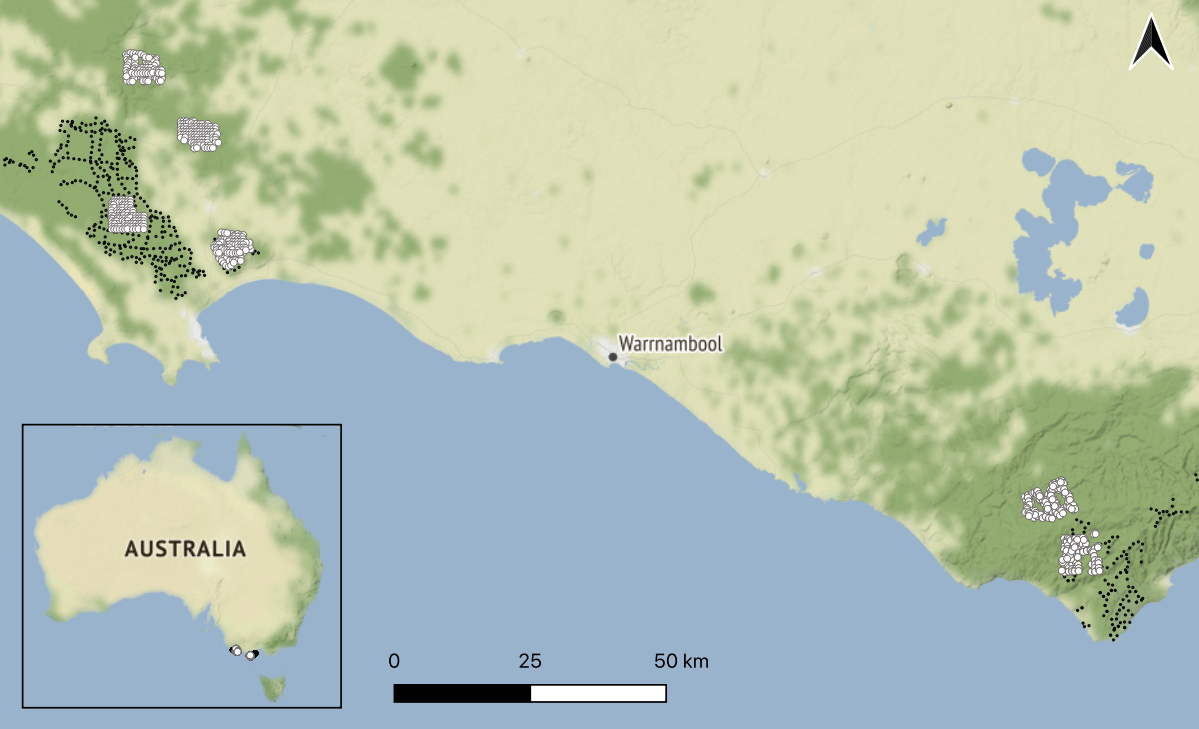
\includegraphics[width=1\linewidth]{figs/fig1} \caption{Locations of our six study landscapes in south-west Victoria, Australia. The location of eight study landscapes are bound in red (note the two Lower Glenelg National Park landscapes in the far west are separated by a river) and the locations of fox poison-bait stations are denoted by black dots. The Glenelg region is to the west and Otway region to the east. Native vegetation is indicated by dark green, with hill shading. \textit{Map tiles by Stamen Design, under CC BY 3.0, map data by OpenStreetMap, under CC BY SA.}}\label{fig:map}
\end{figure}

\newpage

\hypertarget{results}{%
\section{RESULTS}\label{results}}

\hypertarget{fox-occurrence}{%
\subsection{Fox occurrence}\label{fox-occurrence}}

In the Glenelg region, there was a clear difference in fox occurrence between associated impact (poison-baited) and non-impact landscapes for replicates 1 and 3, but only a marginal difference for replicate 2 (Fig. \ref{fig:foxplot}). In the Otway region, fox occurrence in the non-impact landscape increased over the thee years by 22\%, whereas in the impact landscape fox occurrence decreased by 43\% (occurrence probability averaged at each camera-trap in the landscape). Relative to the Glenelg region, fox occurrence in the Otway regions was generally lower, with less fine-scale spatial variation. For example, fox occurrence was predicted to be spatially consistent across the entire Otway region in 2018 (Fig. \ref{fig:foxplot}). Fox model summaries and spatial standard error estimates are presented in Section 5 of the Supporting Information.

\hypertarget{feral-cats-in-the-glenelg-region}{%
\subsection{Feral cats in the Glenelg region}\label{feral-cats-in-the-glenelg-region}}

Across the six landscapes in the Glenelg region, we recorded 251 cat detections from 32,232 camera-trap nights (Table S1). We were able to identify 64\% of cat detections to the individual level; a total of 67 cats (6 -- 13 individuals per landscape). The exponential detector function was supported over the half-normal function (Table S2). The null model was more strongly supported than models with vegetation impacts on cat density and/or linear time trends on \emph{g}\textsubscript{0} (Table S3).

At a fine spatial scale, the model with a linear relationship between fox occurrence and cat density was strongly supported (AICc 2.76 better than the null; Table S4). It indicated that cat density declined as fox occurrence increased (0.73; 95\% CI: 0.57 - 0.93; Fig. \ref{fig:dcor}). Models that included an impact of fox occurrence on cat detectability parameters ranked worse than the null (Table S4). Regression splines added additional model parameters without changing predictions (Fig. \ref{fig:dcor}), and so, all nonlinear models ranked below their linear counterparts (Table S4).

Our hypothesis that cat density would be higher in landscapes with fox control was supported for the first and third replicate pairs: estimated cat density was 2.5 (95\% CI: 1.5 - 4.2) and 3.7 (95\% CI: 1.4 - 9.5) times higher in the impact landscape than the associated non-impact landscape, respectively (Fig. \ref{fig:diffg}). For the second landscape pair, however, the estimated difference was positive but negligible (1.1; 95\% CI: 0.69 - 1.69). At the landscape level, there was some evidence that cat detectability was affected by fox occurrence; however the AICc score was only 0.95 units better than the constant detectability model (Table S5) and the estimated effects were weak with uncertainty high. The detectability of cats in their activity centre (g0) increased with fox occurrence probability (1.27; 95\% CI: 0.72 - 2.2), as did sigma (1.14; 95\% CI: 0.87 - 1.5).

\hypertarget{feral-cats-in-the-otway-region}{%
\subsection{Feral cats in the Otway region}\label{feral-cats-in-the-otway-region}}

In the Otway region, we recorded 970 cat detections from 36,272 camera-trap nights (Table S1). We were able to identify 53\% of cat detections to the individual level; a total of 93 cats (20 -- 30 individuals per landscape). The exponential detector function was strongly supported over the half-normal function (Table S7). The null model was more strongly supported than the models with vegetation impacts on cat density and/or linear time trends on \emph{g}\textsubscript{0} (Table S8).

There was some evidence that cat density was negatively correlated with fox occurrence at a fine spatial scale: the two top-ranked models included a linear and a non-linear effect of fox occurrence on cat density, respectively; however, a model without a fox occurrence term received similar support (dAICc = 0.80; Table S9). The 95\% confidence interval around the linear coefficient from the top-ranked model marginally overlapped one (0.77; 95\% CI: 0.58 - 1.02) indicating that cat density declined as fox occurrence increased in the Otways at a similar rate to Glenelg, but with greater uncertainty (Fig. \ref{fig:dcor}). However, the nonlinear counterpart model predicted cat density to only have declined (at a steeper rate) in mid-high range of fox occurrence probability (Fig. \ref{fig:dcor}). Equivalent pairs of linear model and nonlinear models were indistinguishable based on AICc scores (Table S9).

There was also strong support for an effect of fox occurrence on cat detectability at a fine spatial scale (Fig. \ref{fig:detcor}; Table S9). Where fox occurrence was higher, cats were less detectable in their activity centres (i.e., negative association with g0; 0.50; 95\% CI: 0.33 - -0.76; Fig. \ref{fig:detcor}A) and ranged further (i.e., positive association with sigma; coefficient 1.34; 95\% CI: 1.13 - 1.61; Fig. \ref{fig:detcor}B). However, the nonlinear counterpart of this model predicted detectability changes to have occurred only in the low-mid range of fox occurrence (Fig. \ref{fig:detcor}).

Our hypothesis that cat density in the impact landscape would increase relative to the non-impact landscape with fox control was supported, however there was considerable uncertainty. Cat density tended to be lower in the impact than non-impact landscape prior to fox-baiting (i.e., in 2017), but the confidence intervals for the two density estimates overlapped substantially (Fig. \ref{fig:diffo}). In 2018, cat density decreased in the non-impact landscape and increased in the impact landscape, converging to near-identical density estimates. These patterns continued into 2019, with cat density now somewhat higher in the impact landscape than non-impact landscape. Overlap in the estimated difference for successive years was high, but did suggest a meaningful increase in cat density at the impact landscape from 2017 to 2019 (Fig. \ref{fig:diffo}B). Like the fine scale model, there was strong evidence that cat detectability was impacted by fox occurrence (Table S10).

\newpage

\begin{figure}
\includegraphics[width=1\linewidth]{figs/fig2_600dpi} \caption{Predicted red fox \textit{Vulpes vulpes} occurrence derived from generalised additive models within each impact (I) and associated non-impact (NI) landscape in the Glenelg (a) and Otway (b) regions, Australia. Predicted fox occurrence was used as a predictor of feral cat Felis catus density in the spatial mark-resight models.}\label{fig:foxplot}
\end{figure}

\newpage

\begin{figure}
\includegraphics[width=1\linewidth]{figs/foxD_600dpi} \caption{Linear (solid lines) and nonlinear (dashed lines) models predicted that feral cat \textit{Felis catus} density increased with declining probability of red fox \textit{Vulpes vulpes} occurrence (log-transformed) in the Glenelg and Otway regions, Australia. Shaded areas indicate 95\% confidence intervals.}\label{fig:dcor}
\end{figure}

\newpage

\begin{figure}
\includegraphics[width=1\linewidth]{figs/foxDet_otways_600dpi} \caption{Linear (solid lines) and nonlinear (dashed lines) models of feral cat \textit{Felis catus} detectability as a function of log-transformed red fox \textit{Vulpes vulpes} occurrence in the Otway Ranges, Australia. The probability of detecting a feral cat in its activity centre per 24-hour occasion (\textit{g}\textsubscript{0}) decreased with the probability of fox occurrence (a), while sigma (which is related to home range size; exponential units) increased (b). Shaded areas indicate 95\% confidence intervals.}\label{fig:detcor}
\end{figure}

\newpage

\begin{figure}
\includegraphics[width=1\linewidth]{figs/glenelg_estimates_600dpi} \caption{Landscape-scale feral cat \textit{Felis catus} density estimates (a) and response ratio of cat density in the impact landscape relative to the paired non-impact landscape for each replicate (b) in the Glenelg region, Australia. Poison-baiting for foxes \textit{Vulpes vulpes} has been conducted in the impact landscapes for more than 13 years. Grey dashed line represents no difference between the paired landscapes. Error bars represent 95\% confidence intervals.}\label{fig:diffg}
\end{figure}

\newpage

\begin{figure}
\includegraphics[width=1\linewidth]{figs/otways_estimates_600dpi} \caption{Landscape-scale feral cat \textit{Felis catus} density estimates (a) and response ratio of cat density in the impact landscape relative to the non-impact landscape for each survey year (b) in the Otway region, Australia. In 2017, surveys were conducted approximately two months before lethal red fox \textit{Vulpes vulpes} control commenced in the impact landscape (red); this lapsed for six months prior to the 2018 survey. Grey dashed line represents no difference between the paired landscapes. Error bars represent 95\% confidence intervals.}\label{fig:diffo}
\end{figure}

\newpage

\hypertarget{discussion}{%
\section{DISCUSSION}\label{discussion}}

Our study is one of the first to provide replicated, experimental evidence that apex predator suppression can increase mesopredator population density. Our study provides two lines of evidence that foxes exert top-down control on feral cats: feral cat density was consistently higher where landscape-scale fox control occurred and fine-scale fox occurrence probability was lowest. However, a mesopredator release of feral cats is unlikely to occur universally; fox-cat interactions are context and scale-dependent. More broadly, our study illustrates how correlative and experimental approaches provide complementary lines of evidence when investigating interactions between predator species, and the importance of disentangling changes in population density from changes in detectability.

We were able to exploit a gradient in fox occurrence caused by lethal control to investigate associations between cat density and fox occurrence at a fine spatial scale across two separate regions. At this scale, we observed a similar negative association between cat density and fox occurrence in each region, although there was more uncertainty around the relationship in the Otway region. Across the gradient of fox occurrence, overall cat density was consistently higher in the Otway region than Glenelg, likely reflecting relatively high small mammal (i.e., prey) abundance (Rees \emph{et al.} 2019) and lower fox occurrence at the landscape-level. Rather than avoidance or exclusion, the negative correlation between foxes and cats we observed could simply reflect differences in niche preference. However, this is unlikely because we observed the relationship across an artificial gradient of fox occurrence caused by lethal control.

There is contention around whether linear regression is appropriate for investigating correlations between different predator species, as subordinate predators may only be suppressed when apex predator abundance is high (Johnson \& VanDerWal 2009). We found no evidence of non-linear associations between foxes and cats in the Glenelg region, while linear and non-linear models performed equally well in the Otway region. Non-linear models in the Otway region predicted that cat density declined only in the mid-high range of fox occurrence, while behavioural changes were seen in the low-mid range of fox occurrence. Perhaps cats can successfully avoid foxes through behavioural change where foxes are rare, but this is ineffective where foxes are common. Fox avoidance strategies likely come at the expense of hunting success (Sih 1980), which may mean that they are untenable for cats in the Glenelg region where small mammal abundance is relatively low (Wilson \emph{et al.} 2010).

Where fox occurrence was higher in the Otway Ranges, cats were less detectable in their activity centres and ranged further (Fig. \ref{fig:detcor}). Low detectability is likely to correlate with fewer apex predator encounters, and has been observed in other predator interaction studies (e.g.~Lombardi \emph{et al.} 2017). An increase in cat ranging behaviour (sigma) with fox control supports observations made by Molsher \emph{et al.} (2017), and may reflect a direct avoidance strategy. Animal movement rates are expected to increase in response to unpredictable threats (Riotte-Lambert \& Matthiopoulos 2020). Alternatively, cats may consider foxes predictable and avoid locations they frequent, thus having to range further to obtain the same amount of food resources. In a similar forest habitat, Buckmaster (2012) observed large `holes' in the home range of each GPS-collared cat; they confirmed that this was not due to an absence of prey and hypothesised that it could be due to apex predator avoidance. Regardless of the cause, variation in mesopredator detectability and movement rates with apex predator populations has serious implications for the interpretation of studies that compare relative abundance indices and spatial overlap of predator species without disentangling behaviour and detectability from density (Efford \& Dawson 2012; Neilson \emph{et al.} 2018; Stewart \emph{et al.} 2018; Broadley \emph{et al.} 2019).

In the Glenelg region where fox-baiting had occurred for more than 13 years, feral cat density was considerably higher in two out of three distinct landscapes relative to similar, unbaited landscapes. The outlier is most likely due to limited suppression of foxes at Mt Clay (Fig. \ref{fig:foxplot}), a small forest block surrounded entirely by unbaited farmland. Simulation modelling indicates that the size of the baited area is a key driver of the degree of reduction in the fox population (Hradsky \emph{et al.} 2019; Francis \emph{et al.} 2020). Studies of fox-cat (and other predator-predator) interactions often use the presence of a management program as a proxy for lower apex predator abundance and distribution (e.g.~Hunter \emph{et al.} 2018). Our findings strongly indicate the need to directly measure the apex predator population in order to reliably interpret the responses of subordinate species (Salo \emph{et al.} 2010).

In the Otway region, we observed a weaker--but increasing--effect of fox control on cat density, to be expected from a recently commenced and less intensive fox-baiting program. The short duration of baiting in the Otway region may mean that changes in adult cat density are yet to fully manifest; foxes potentially suppress cats by reducing recruitment rates (Ritchie \& Johnson 2009). Cats may also respond to an increase in shared prey availability following fox suppression (Stobo-Wilson \emph{et al.} 2020). A time-lagged release of cats following fox control would explain eruptions and subsequent crashes commonly observed in shared mammalian prey populations two to ten years following fox control commencement (Duncan \emph{et al.} 2020). Alternatively, top-down suppression by foxes and competition may be weaker in this highly productive environment where fox occurrence was already relatively low (Johnson \& VanDerWal 2009; Greenville \emph{et al.} 2014). Our surveys provide an important baseline against which to compare future changes in predator populations as the fox-baiting program continues.

Our study is among the very few which have used a direct measure of density to test mesopredator release. Previous studies have mostly used live capture-rates to infer population density, without accounting for behavioural or detectability changes (e.g.~Arjo \emph{et al.} 2007; Karki \emph{et al.} 2007; Thompson \& Gese 2007; Berger \emph{et al.} 2008; Jones \emph{et al.} 2008). Contention about mesopredator release has centred on such methods (Hayward \& Marlow 2014); as well as unaccounted species interactions in complex predator guilds (Levi \& Wilmers 2012; Jachowski \emph{et al.} 2020). In contrast, our study tests the mesopredator release theory using a combined behavioural and numerical approach, in a system with a simplified carnivore guild. One limitation of our approach is that uncertainty from our fox occurrence models was not propagated into the spatial mark-resight models. A full Bayesian integration of the fox occurrence analysis and the spatial mark-resight model to address this is not yet implemented. The development of open population spatial mark-resight models would also improve parameter estimates for multi-season surveys.

The results of our study may explain why pest management that only targets foxes--one of the most prevalent conservation actions in Australia--does not consistently improve native prey persistence (Dexter \& Murray 2009; Robley \emph{et al.} 2014; Wayne \emph{et al.} 2017; Lindenmayer \emph{et al.} 2018; Duncan \emph{et al.} 2020). However, more evidence is required to understand the circumstances in which lethal fox control increases cat density, particularly the role of prey. A more integrated approach to invasive predator management, where foxes and cats are simultaneously or otherwise optimally controlled could substantially improve biodiversity outcomes (Risbey \emph{et al.} 2000; Comer \emph{et al.} 2020). If this is not feasible, changes in invasive mesopredator density and the outcomes for native prey species should be closely monitored as part of any control program for invasive apex predators, with triggers for ceasing apex predator control or commencing integrated management if single-species control proves counterproductive for the conservation of threatened prey species.

\newpage

\hypertarget{acknowledgements}{%
\section{ACKNOWLEDGEMENTS}\label{acknowledgements}}

We acknowledge and pay respect to the Gadubanud and Gunditjmara peoples on whose traditional lands this study took place. Surveys were conducted under University of Melbourne Animal Ethics Committee approval 1714119 and Victorian Government Department of Environment, Land Water and Planning Research Permit 10008273. This experiment was conducted in cooperation with the Glenelg Ark (Department of Environment, Land Water and Planning) and Otway Ark (Parks Victoria) working groups. Ethan Le Duc, Michael Murrell, Dylan Thomas, Rhys Weber, Chris Johansson, Lachlan Levings and Liz Beever carried out the Lower Glenelg National Park surveys, with Luke Woodford identifying cats here. We are extremely grateful to our field assistants: Shauni Omond, Shayne Neal, Asitha Samarawickrama, Shelley Thompson, Erin Harris, Hannah Killian, Lani Watson, Mark Dorman, Jack Davis, Carl Roffey, Bruce Edley, Larissa Oliveira Gonçalves, Ben Lake, Chantelle Geissler, Aviya Naccarella, Emily Gronow, Harley England, David Pitts, Annie Hobby, Louise Falls, Thomas McKinnon, Jimmy Downie, Marney Hradsky, Stephanie Samson, Robin Sinclair, Asmaa Alhusainan, Kelly Forrester, Tammana Wadawani, Emily McColl-Gausden, Emily Gregg, Hannah Edwards, Adam Beck, Vishnu Memnon, Sandy Lu, Dr Pia Lentini, Prof.~Nick Golding, Emily McColl-Gausden, Nina Page, Maggie Campbell-Jones, Kyle Quinn and Jack Dickson. This manuscript was improved by comments from William Geary; Dr Joanne Potts also gave instrumental advice on fitting spatial mark-resight models. Our study was generously supported by the Conservation Ecology Centre, the Victorian Government Department of Environment, Land Water and Planning, Arthur Rylah Institute for Environmental Research, Parks Victoria, the Australian Government's National Environmental Science Program through the Threatened Species Recovery Hub, and ARC Linkage Project LP170101134. M.W.R also receives support from an Australian Government Research Training Program Scholarship.

\hypertarget{authorship}{%
\section{AUTHORSHIP}\label{authorship}}

M.W.R, B.A.H, J.H.P, B.A.W and A.R conceived the ideas and designed the methodology; M.W.R, J.H.P, M.LP, E.K.B and B.A.H collected the data; M.W.R analysed the data with input from B.A.H and B.A.W, and led the writing of the manuscript. All authors contributed critically to the drafts and gave final approval for publication.

\hypertarget{open-research}{%
\section{OPEN RESEARCH}\label{open-research}}

Data and code will be deposited on the Dryad Digital Repository after acceptance and can be viewed at this \href{https://github.com/matt-w-rees/C2_cat_density}{GitHub link}.

\newpage

\hypertarget{references}{%
\section*{REFERENCES}\label{references}}
\addcontentsline{toc}{section}{REFERENCES}

\hypertarget{refs}{}
\leavevmode\hypertarget{ref-alston2019}{}%
Alston, J., Maitland, B., Brito, B., Esmaeili, S., Ford, A. \& Hays, B. \emph{et al.} (2019). Reciprocity in restoration ecology: When might large carnivore reintroduction restore ecosystems? \emph{Biological conservation}, 234, 82--89.

\leavevmode\hypertarget{ref-arjo2007}{}%
Arjo, W.M., Gese, E.M., Bennett, T.J. \& Kozlowski, A.J. (2007). Changes in kit fox--coyote--prey relationships in the Great Basin Desert, Utah. \emph{Western North American Naturalist}, 67, 389--401.

\leavevmode\hypertarget{ref-ballari2016}{}%
Ballari, S.A., Kuebbing, S.E. \& Nuñez, M.A. (2016). Potential problems of removing one invasive species at a time: A meta-analysis of the interactions between invasive vertebrates and unexpected effects of removal programs. \emph{PeerJ}, 4, e2029.

\leavevmode\hypertarget{ref-berger2008indirect}{}%
Berger, K.M., Gese, E.M. \& Berger, J. (2008). Indirect effects and traditional trophic cascades: A test involving wolves, coyotes, and pronghorn. \emph{Ecology}, 89, 818--828.

\leavevmode\hypertarget{ref-bode2015}{}%
Bode, M., Baker, C.M. \& Plein, M. (2015). Eradicating down the food chain: Optimal multispecies eradication schedules for a commonly encountered invaded island ecosystem. \emph{Journal of Applied Ecology}, 52, 571--579.

\leavevmode\hypertarget{ref-borchers2008}{}%
Borchers, D.L. \& Efford, M.G. (2008). Spatially explicit maximum likelihood methods for capture--recapture studies. \emph{Biometrics}, 64, 377--385.

\leavevmode\hypertarget{ref-broadley2019}{}%
Broadley, K., Burton, A.C., Avgar, T. \& Boutin, S. (2019). Density-dependent space use affects interpretation of camera trap detection rates. \emph{Ecology and evolution}, 9, 14031--14041.

\leavevmode\hypertarget{ref-2123-8123}{}%
Buckmaster, A.J. (2012). Ecology of the feral cat (felis catus) in the tall forests of far east gippsland. PhD thesis. University of Sydney.; School of Biological Sciences; University of Sydney.; School of Biological Sciences.

\leavevmode\hypertarget{ref-BOM2021}{}%
\emph{Bureau of meteorology}. (2021). \emph{Climate Data Online URL}. Available at: \url{http://www.bom.gov.au/climate/data/}. Last accessed.

\leavevmode\hypertarget{ref-burnham2004}{}%
Burnham, K.P. \& Anderson, D.R. (2004). Multimodel inference: Understanding aic and bic in model selection. \emph{Sociological methods \& research}, 33, 261--304.

\leavevmode\hypertarget{ref-10.2307ux2f23566419}{}%
Chandler, R.B. \& Royle, J.A. (2013). Spatially explicit models for inference about density in unmarked or partially marked populations. \emph{The Annals of Applied Statistics}, 7, 936--954.

\leavevmode\hypertarget{ref-christie2019}{}%
Christie, A.P., Amano, T., Martin, P.A., Shackelford, G.E., Simmons, B.I. \& Sutherland, W.J. (2019). Simple study designs in ecology produce inaccurate estimates of biodiversity responses. \emph{Journal of Applied Ecology}, 56, 2742--2754.

\leavevmode\hypertarget{ref-claridge2010}{}%
Claridge, A.W., Cunningham, R.B., Catling, P.C. \& Reid, A.M. (2010). Trends in the activity levels of forest-dwelling vertebrate fauna against a background of intensive baiting for foxes. \emph{Forest Ecology and Management}, 260, 822--832.

\leavevmode\hypertarget{ref-comer2020integrating}{}%
Comer, S., Clausen, L., Cowen, S., Pinder, J., Thomas, A. \& Burbidge, A.H. \emph{et al.} (2020). Integrating feral cat (felis catus) control into landscape-scale introduced predator management to improve conservation prospects for threatened fauna: A case study from the south coast of western australia. \emph{Wildlife Research}, 47, 762--778.

\leavevmode\hypertarget{ref-courchamp1999}{}%
Courchamp, F., Langlais, M. \& Sugihara, G. (1999). Cats protecting birds: Modelling the mesopredator release effect. \emph{Journal of Animal Ecology}, 68, 282--292.

\leavevmode\hypertarget{ref-crooks1999}{}%
Crooks, K.R. \& Soulé, M.E. (1999). Mesopredator release and avifaunal extinctions in a fragmented system. \emph{Nature}, 400, 563--566.

\leavevmode\hypertarget{ref-cumming2005inference}{}%
Cumming, G. \& Finch, S. (2005). Inference by eye: Confidence intervals and how to read pictures of data. \emph{American psychologist}, 60, 170.

\leavevmode\hypertarget{ref-davey2006}{}%
Davey, C., Sinclair, A., Pech, R.P., Arthur, A.D., Krebs, C.J. \& Newsome, A. \emph{et al.} (2006). Do exotic vertebrates structure the biota of australia? An experimental test in new south wales. \emph{Ecosystems}, 9, 992--1008.

\leavevmode\hypertarget{ref-dexter2009impact}{}%
Dexter, N. \& Murray, A. (2009). The impact of fox control on the relative abundance of forest mammals in east gippsland, victoria. \emph{Wildlife Research}, 36, 252--261.

\leavevmode\hypertarget{ref-doherty2017}{}%
Doherty, T.S. \& Ritchie, E.G. (2017). Stop jumping the gun: A call for evidence-based invasive predator management. \emph{Conservation Letters}, 10, 15--22.

\leavevmode\hypertarget{ref-duncan2020eruptive}{}%
Duncan, R.P., Dexter, N., Wayne, A. \& Hone, J. (2020). Eruptive dynamics are common in managed mammal populations. \emph{Ecology}, 101, e03175.

\leavevmode\hypertarget{ref-efford2021secr}{}%
Efford, M.G. (2021). \emph{Secr: Spatially explicit capture-recapture models. R package version 4.4.4}. Available at: \url{http://CRAN.R-project.org/package=secr}. Last accessed.

\leavevmode\hypertarget{ref-efford2012}{}%
Efford, M.G. \& Dawson, D.K. (2012). Occupancy in continuous habitat. \emph{Ecosphere}, 3, 1--15.

\leavevmode\hypertarget{ref-https:ux2fux2fdoi.orgux2f10.1890ux2f13-1497.1}{}%
Efford, M.G. \& Mowat, G. (2014). Compensatory heterogeneity in spatially explicit capture--recapture data. \emph{Ecology}, 95, 1341--1348.

\leavevmode\hypertarget{ref-finke2004}{}%
Finke, D.L. \& Denno, R.F. (2004). Predator diversity dampens trophic cascades. \emph{Nature}, 429, 407--410.

\leavevmode\hypertarget{ref-fisher2015}{}%
Fisher, P., Algar, D., Murphy, E., Johnston, M. \& Eason, C. (2015). How does cat behaviour influence the development and implementation of monitoring techniques and lethal control methods for feral cats? \emph{Applied Animal Behaviour Science}, 173, 88--96.

\leavevmode\hypertarget{ref-francis2020evaluating}{}%
Francis, L., Robley, A. \& Hradsky, B. (2020). Evaluating fox management strategies using a spatially explicit population. \emph{Arthur Rylah Institute for Environmental Research Technical Report Series No. 304. Department of Environment, Land, Water and Planning, Heidelberg, Victoria}.

\leavevmode\hypertarget{ref-glen2005}{}%
Glen, A.S. \& Dickman, C.R. (2005). Complex interactions among mammalian carnivores in australia, and their implications for wildlife management. \emph{Biological reviews}, 80, 387--401.

\leavevmode\hypertarget{ref-greenville2014bottom}{}%
Greenville, A.C., Wardle, G.M., Tamayo, B. \& Dickman, C.R. (2014). Bottom-up and top-down processes interact to modify intraguild interactions in resource-pulse environments. \emph{Oecologia}, 175, 1349--1358.

\leavevmode\hypertarget{ref-hastings2001}{}%
Hastings, A. (2001). Transient dynamics and persistence of ecological systems. \emph{Ecology Letters}, 4, 215--220.

\leavevmode\hypertarget{ref-hayward2015}{}%
Hayward, M.W., Boitani, L., Burrows, N.D., Funston, P.J., Karanth, K.U. \& MacKenzie, D.I. \emph{et al.} (2015). Ecologists need robust survey designs, sampling and analytical methods. \emph{Journal of Applied Ecology}, 52, 286--290.

\leavevmode\hypertarget{ref-https:ux2fux2fdoi.orgux2f10.1111ux2f1365-2664.12250}{}%
Hayward, M.W. \& Marlow, N. (2014). Will dingoes really conserve wildlife and can our methods tell? \emph{Journal of Applied Ecology}, 51, 835--838.

\leavevmode\hypertarget{ref-hradsky2019foxnet}{}%
Hradsky, B.A., Kelly, L.T., Robley, A. \& Wintle, B.A. (2019). FoxNet: An individual-based model framework to support management of an invasive predator, the red fox. \emph{Journal of Applied Ecology}, 56, 1460--1470.

\leavevmode\hypertarget{ref-hradsky2017human}{}%
Hradsky, B.A., Robley, A., Alexander, R., Ritchie, E.G., York, A. \& Di Stefano, J. (2017). Human-modified habitats facilitate forest-dwelling populations of an invasive predator, vulpes vulpes. \emph{Scientific Reports}, 7, 1--12.

\leavevmode\hypertarget{ref-hunter2018}{}%
Hunter, D.O., Lagisz, M., Leo, V., Nakagawa, S. \& Letnic, M. (2018). Not all predators are equal: A continent-scale analysis of the effects of predator control on australian mammals. \emph{Mammal Review}, 48, 108--122.

\leavevmode\hypertarget{ref-https:ux2fux2fdoi.orgux2f10.1111ux2fmam.12207}{}%
Jachowski, D.S., Butler, A., Eng, R.Y.Y., Gigliotti, L., Harris, S. \& Williams, A. (2020). Identifying mesopredator release in multi-predator systems: A review of evidence from north america. \emph{Mammal Review}, 50, 367--381.

\leavevmode\hypertarget{ref-jackson2015}{}%
Jackson, M.C. (2015). Interactions among multiple invasive animals. \emph{Ecology}, 96, 2035--2041.

\leavevmode\hypertarget{ref-https:ux2fux2fdoi.orgux2f10.1111ux2fj.1365-2664.2009.01650.x}{}%
Johnson, C.N. \& VanDerWal, J. (2009). Evidence that dingoes limit abundance of a mesopredator in eastern australian forests. \emph{Journal of Applied Ecology}, 46, 641--646.

\leavevmode\hypertarget{ref-jones2008sudden}{}%
Jones, K.L., Van Vuren, D.H. \& Crooks, K.R. (2008). Sudden Increase in a Rare Endemic Carnivore: Ecology of the Island Spotted Skunk. \emph{Journal of Mammalogy}, 89, 75--86.

\leavevmode\hypertarget{ref-karki2007}{}%
Karki, S.M., Gese, E.M. \& Klavetter, M.L. (2007). Effects of coyote population reduction on swift fox demographics in southeastern colorado. \emph{The Journal of Wildlife Management}, 71, 2707--2718.

\leavevmode\hypertarget{ref-kuebbing2015}{}%
Kuebbing, S.E. \& Nuñez, M.A. (2015). Negative, neutral, and positive interactions among nonnative plants: Patterns, processes, and management implications. \emph{Global Change Biology}, 21, 926--934.

\leavevmode\hypertarget{ref-lazenby2015}{}%
Lazenby, B.T., Mooney, N.J. \& Dickman, C.R. (2015). Effects of low-level culling of feral cats in open populations: A case study from the forests of southern tasmania. \emph{Wildlife Research}, 41, 407--420.

\leavevmode\hypertarget{ref-legge2020}{}%
Legge, S., Taggart, P.L., Dickman, C.R., Read, J.L. \& Woinarski, J.C. (2020). \emph{Wildlife Research}, 47, 731--746.

\leavevmode\hypertarget{ref-https:ux2fux2fdoi.orgux2f10.1890ux2f11-0165.1}{}%
Levi, T. \& Wilmers, C.C. (2012). Wolves--coyotes--foxes: A cascade among carnivores. \emph{Ecology}, 93, 921--929.

\leavevmode\hypertarget{ref-LINDENMAYER2018279}{}%
Lindenmayer, D.B., Wood, J., MacGregor, C., Foster, C., Scheele, B. \& Tulloch, A. \emph{et al.} (2018). Conservation conundrums and the challenges of managing unexplained declines of multiple species. \emph{Biological Conservation}, 221, 279--292.

\leavevmode\hypertarget{ref-lombardi2017coyote}{}%
Lombardi, J.V., Comer, C.E., Scognamillo, D.G. \& Conway, W.C. (2017). Coyote, fox, and bobcat response to anthropogenic and natural landscape features in a small urban area. \emph{Urban Ecosystems}, 20, 1239--1248.

\leavevmode\hypertarget{ref-marlow2015}{}%
Marlow, N.J., Thomas, N.D., Williams, A.A., Macmahon, B., Lawson, J. \& Hitchen, Y. \emph{et al.} (2015). Cats (felis catus) are more abundant and are the dominant predator of woylies (bettongia penicillata) after sustained fox (vulpes vulpes) control. \emph{Australian Journal of Zoology}, 63, 18--27.

\leavevmode\hypertarget{ref-mcleod2014}{}%
McLeod, S.R. \& Saunders, G. (2014). Fertility control is much less effective than lethal baiting for controlling foxes. \emph{Ecological Modelling}, 273, 1--10.

\leavevmode\hypertarget{ref-medina2011}{}%
Medina, F.M., Bonnaud, E., Vidal, E., Tershy, B.R., Zavaleta, E.S. \& Josh Donlan, C. \emph{et al.} (2011). A global review of the impacts of invasive cats on island endangered vertebrates. \emph{Global Change Biology}, 17, 3503--3510.

\leavevmode\hypertarget{ref-miller2014}{}%
Miller, D.L. \& Wood, S.N. (2014). Finite area smoothing with generalized distance splines. \emph{Environmental and ecological statistics}, 21, 715--731.

\leavevmode\hypertarget{ref-molsher2017}{}%
Molsher, R., Newsome, A.E., Newsome, T.M. \& Dickman, C.R. (2017). Mesopredator management: Effects of red fox control on the abundance, diet and use of space by feral cats. \emph{PLoS One}, 12, e0168460.

\leavevmode\hypertarget{ref-moseby2019}{}%
Moseby, K.E., Letnic, M., Blumstein, D.T. \& West, R. (2019). Understanding predator densities for successful co-existence of alien predators and threatened prey. \emph{Austral Ecology}, 44, 409--419.

\leavevmode\hypertarget{ref-moseby2020effectiveness}{}%
Moseby, K., McGregor, H. \& Read, J. (2020). Effectiveness of the felixer grooming trap for the control of feral cats: A field trial in arid south australia. \emph{Wildlife Research}, 47, 599--609.

\leavevmode\hypertarget{ref-https:ux2fux2fdoi.orgux2f10.1002ux2fecs2.2092}{}%
Neilson, E.W., Avgar, T., Burton, A.C., Broadley, K. \& Boutin, S. (2018). Animal movement affects interpretation of occupancy models from camera-trap surveys of unmarked animals. \emph{Ecosphere}, 9, e02092.

\leavevmode\hypertarget{ref-rayner2007}{}%
Rayner, M.J., Hauber, M.E., Imber, M.J., Stamp, R.K. \& Clout, M.N. (2007). Spatial heterogeneity of mesopredator release within an oceanic island system. \emph{Proceedings of the National Academy of Sciences}, 104, 20862--20865.

\leavevmode\hypertarget{ref-reddiex2007}{}%
Reddiex, B., Forsyth, D.M., McDonald-Madden, E., Einoder, L.D., Griffioen, P.A. \& Chick, R.R. \emph{et al.} (2007). Control of pest mammals for biodiversity protection in australia. I. Patterns of control and monitoring. \emph{Wildlife Research}, 33, 691--709.

\leavevmode\hypertarget{ref-rees2019}{}%
Rees, M., Pascoe, J., Wintle, B., Le Pla, M., Birnbaum, E. \& Hradsky, B. (2019). Unexpectedly high densities of feral cats in a rugged temperate forest. \emph{Biological Conservation}, 239, 108287.

\leavevmode\hypertarget{ref-riley1999}{}%
Riley, S.J., DeGloria, S.D. \& Elliot, R. (1999). Index that quantifies topographic heterogeneity. \emph{intermountain Journal of sciences}, 5, 23--27.

\leavevmode\hypertarget{ref-RIOTTELAMBERT2020163}{}%
Riotte-Lambert, L. \& Matthiopoulos, J. (2020). Environmental predictability as a cause and consequence of animal movement. \emph{Trends in Ecology \& Evolution}, 35, 163--174.

\leavevmode\hypertarget{ref-risbey2000}{}%
Risbey, D.A., Calver, M.C., Short, J., Bradley, J.S. \& Wright, I.W. (2000). The impact of cats and foxes on the small vertebrate fauna of heirisson prong, western australia. II. A field experiment. \emph{Wildlife Research}, 27, 223--235.

\leavevmode\hypertarget{ref-ritchie2009predator}{}%
Ritchie, E.G. \& Johnson, C.N. (2009). Predator interactions, mesopredator release and biodiversity conservation. \emph{Ecology Letters}, 12, 982--998.

\leavevmode\hypertarget{ref-robley2014}{}%
Robley, A., Gormley, A.M., Forsyth, D.M. \& Triggs, B. (2014). Long-term and large-scale control of the introduced red fox increases native mammal occupancy in australian forests. \emph{Biological Conservation}, 180, 262--269.

\leavevmode\hypertarget{ref-rogan2019}{}%
Rogan, M.S., Balme, G.A., Distiller, G., Pitman, R.T., Broadfield, J. \& Mann, G.K. \emph{et al.} (2019). The influence of movement on the occupancy--density relationship at small spatial scales. \emph{Ecosphere}, 10, e02807.

\leavevmode\hypertarget{ref-ruscoe2011}{}%
Ruscoe, W.A., Ramsey, D.S., Pech, R.P., Sweetapple, P.J., Yockney, I. \& Barron, M.C. \emph{et al.} (2011). Unexpected consequences of control: Competitive vs. Predator release in a four-species assemblage of invasive mammals. \emph{Ecology Letters}, 14, 1035--1042.

\leavevmode\hypertarget{ref-https:ux2fux2fdoi.orgux2f10.1890ux2f09-1260.1}{}%
Salo, P., Banks, P.B., Dickman, C.R. \& Korpimäki, E. (2010). Predator manipulation experiments: Impacts on populations of terrestrial vertebrate prey. \emph{Ecological Monographs}, 80, 531--546.

\leavevmode\hypertarget{ref-SIH1041}{}%
Sih, A. (1980). Optimal behavior: Can foragers balance two conflicting demands? \emph{Science}, 210, 1041--1043.

\leavevmode\hypertarget{ref-smith2020}{}%
Smith, J.A., Suraci, J.P., Hunter, J.S., Gaynor, K.M., Keller, C.B. \& Palmer, M.S. \emph{et al.} (2020). Zooming in on mechanistic predator--prey ecology: Integrating camera traps with experimental methods to reveal the drivers of ecological interactions. \emph{Journal of Animal Ecology}, 89, 1997--2012.

\leavevmode\hypertarget{ref-soule1988}{}%
Soulé, M.E., Bolger, D.T., Alberts, A.C., Wrights, J., Sorice, M. \& Hill, S. (1988). Reconstructed dynamics of rapid extinctions of chaparral-requiring birds in urban habitat islands. \emph{Conservation Biology}, 2, 75--92.

\leavevmode\hypertarget{ref-stephens2015}{}%
Stephens, P.A., Pettorelli, N., Barlow, J., Whittingham, M.J. \& Cadotte, M.W. (2015). Management by proxy? The use of indices in applied ecology.

\leavevmode\hypertarget{ref-stewart2018}{}%
Stewart, F.E.C., Fisher, J.T., Burton, A.C. \& Volpe, J.P. (2018). Species occurrence data reflect the magnitude of animal movements better than the proximity of animal space use. \emph{Ecosphere}, 9, e02112.

\leavevmode\hypertarget{ref-stobo2020management}{}%
Stobo-Wilson, A.M., Brandle, R., Johnson, C.N. \& Jones, M.E. (2020). Management of invasive mesopredators in the flinders ranges, south australia: Effectiveness and implications. \emph{Wildlife Research}, 47, 720--730.

\leavevmode\hypertarget{ref-STOBOWILSON2021109284}{}%
Stobo-Wilson, A.M., Murphy, B.P., Crawford, H.M., Dawson, S.J., Dickman, C.R. \& Doherty, T.S. \emph{et al.} (2021a). Sharing meals: Predation on australian mammals by the introduced european red fox compounds and complements predation by feral cats. \emph{Biological Conservation}, 261, 109284.

\leavevmode\hypertarget{ref-stobo2021reptiles}{}%
Stobo-Wilson, A.M., Murphy, B.P., Legge, S.M., Chapple, D.G., Crawford, H.M. \& Dawson, S.J. \emph{et al.} (2021b). Reptiles as food: Predation of australian reptiles by introduced red foxes compounds and complements predation by cats. \emph{Wildlife Research}.

\leavevmode\hypertarget{ref-thompson2007food}{}%
Thompson, C.M. \& Gese, E.M. (2007). Food webs and intraguild predation: Community interactions of a native mesocarnivore. \emph{Ecology}, 88, 334--346.

\leavevmode\hypertarget{ref-towerton2011}{}%
Towerton, A.L., Penman, T.D., Kavanagh, R.P. \& Dickman, C.R. (2011). Detecting pest and prey responses to fox control across the landscape using remote cameras. \emph{Wildlife Research}, 38, 208--220.

\leavevmode\hypertarget{ref-wayne2017recoveries}{}%
Wayne, A.F., Maxwell, M.A., Ward, C.G., Wayne, J.C., Vellios, C.V. \& Wilson, I.J. (2017). Recoveries and cascading declines of native mammals associated with control of an introduced predator. \emph{Journal of Mammalogy}, 98, 489--501.

\leavevmode\hypertarget{ref-wilson2010prey}{}%
Wilson, R.R., Blankenship, T.L., Hooten, M.B. \& Shivik, J.A. (2010). Prey-mediated avoidance of an intraguild predator by its intraguild prey. \emph{Oecologia}, 164, 921--929.

\leavevmode\hypertarget{ref-Woinarski4531}{}%
Woinarski, J.C.Z., Burbidge, A.A. \& Harrison, P.L. (2015). Ongoing unraveling of a continental fauna: Decline and extinction of australian mammals since european settlement. \emph{Proceedings of the National Academy of Sciences}, 112, 4531--4540.

\leavevmode\hypertarget{ref-wood2011}{}%
Wood, S.N. (2011). Fast stable restricted maximum likelihood and marginal likelihood estimation of semiparametric generalized linear models. \emph{Journal of the Royal Statistical Society: Series B (Statistical Methodology)}, 73, 3--36.

\leavevmode\hypertarget{ref-wood2017}{}%
Wood, S.N. (2017). \emph{Generalized additive models: An introduction with r}. CRC press.

\leavevmode\hypertarget{ref-zavaleta2001}{}%
Zavaleta, E.S., Hobbs, R.J. \& Mooney, H.A. (2001). Viewing invasive species removal in a whole-ecosystem context. \emph{Trends in Ecology \& Evolution}, 16, 454--459.


\end{document}


